\section{Physics Informed Neural Networks(PINNs)}


\begin{frame}{From Data-Driven to Physics-Driven Learning}
  The Limitations of Purely Data-Driven Models
  \begin{itemize}
    \item Require large, high-quality datasets
    \item Perform poorly when data are scarce or noisy
    \item May violate physical laws (e.g., conservation of mass, energy, momentum)
  \end{itemize}
  Motivation for Physics-Guided Learning
  \begin{itemize}
    \item In scientific problems, data are limited but laws are known
    \item Use domain knowledge (PDEs, constraints) to guide learning
    \item Integrate physics directly into the loss function
    \item Learn from both data + physics instead of data alone
  \end{itemize}
\end{frame}

\begin{frame}{PINNs}
  \begin{center}

    \begin{figure}
    \centering
    \includegraphics[width=0.85\textwidth]{images/Screenshot 2025-11-01 212541.png}
  \end{figure}

  \end{center}
\end{frame}


\begin{frame}{Naive NN}

\begin{center}

  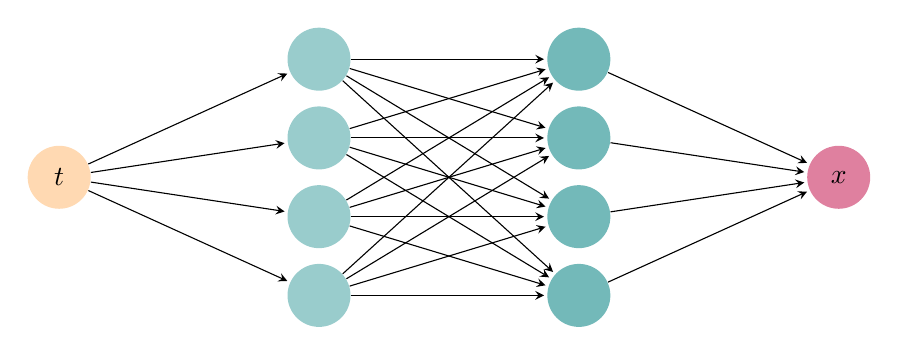
\begin{tikzpicture}[>=stealth, x=2.2cm, y=1cm]
\centering
% Parameters
\def\inputnum{1}
\def\hiddennum{4}
\def\outputnum{1}

% === Input Layer ===
\foreach \i in {1,...,\inputnum}{
  \node[circle, minimum size=8mm, fill=orange!30] 
    (Input-\i) at (0,-\i-1) {$t$};
}

% === Hidden Layer 1 ===
\foreach \i in {1,...,\hiddennum}{
  \node[circle, minimum size=8mm, fill=teal!40] 
    (HiddenA-\i) at (1.5,-\i + 0.5) {};
}

% === Hidden Layer 2 ===
\foreach \i in {1,...,\hiddennum}{
  \node[circle, minimum size=8mm, fill=teal!55] 
    (HiddenB-\i) at (3,-\i + 0.5) {};
}



% === Output Layer ===
\foreach \i in {1,...,\outputnum}{
  \node[circle, minimum size=8mm, fill=purple!50]
    (Output-\i) at (4.5,-\i-1) {$x$};
}

% === Connections ===
% Input → Hidden 1
\foreach \i in {1,...,\inputnum}{
  \foreach \j in {1,...,\hiddennum}{
    \draw[->, shorten >=1pt] (Input-\i) -- (HiddenA-\j);
  }
}

% Hidden 1 → Hidden 2
\foreach \i in {1,...,\hiddennum}{
  \foreach \j in {1,...,\hiddennum}{
    \draw[->, shorten >=1pt] (HiddenA-\i) -- (HiddenB-\j);
  }
}



% Hidden 3 → Output
\foreach \i in {1,...,\hiddennum}{
  \foreach \j in {1,...,\outputnum}{
    \draw[->, shorten >=1pt] (HiddenB-\i) -- (Output-\j);
  }
}

% % === Labels ===
% \node[above] at (0,0) {Input Layer};
% \node[above] at (1.5,0) {Hidden 1};
% \node[above] at (3,0) {Hidden 2};
% \node[above] at (4.6,0) {Hidden 3};
% \node[above] at (6,0) {Output Layer};
\end{tikzpicture}

$$ \text{Loss} = \frac{1}{N}\sum_{i}^{N}\left(x_{\text{nn}}(t_i)- x_{\text{true}}(t_i)\right)^2$$

\pause
  \begin{figure}
    \includegraphics[width=0.7\linewidth]{images/nn/nn-0.jpg}
\end{figure}
\end{center}
\end{frame}

% \begin{frame}{Naive NN}

% \begin{center}

%   \begin{tikzpicture}[>=stealth, x=2.2cm, y=1cm]
% \centering
% % Parameters
% \def\inputnum{1}
% \def\hiddennum{4}
% \def\outputnum{1}

% % === Input Layer ===
% \foreach \i in {1,...,\inputnum}{
%   \node[circle, minimum size=8mm, fill=orange!30] 
%     (Input-\i) at (0,-\i-1) {$t$};
% }

% % === Hidden Layer 1 ===
% \foreach \i in {1,...,\hiddennum}{
%   \node[circle, minimum size=8mm, fill=teal!40] 
%     (HiddenA-\i) at (1.5,-\i + 0.5) {};
% }

% % === Hidden Layer 2 ===
% \foreach \i in {1,...,\hiddennum}{
%   \node[circle, minimum size=8mm, fill=teal!55] 
%     (HiddenB-\i) at (3,-\i + 0.5) {};
% }



% % === Output Layer ===
% \foreach \i in {1,...,\outputnum}{
%   \node[circle, minimum size=8mm, fill=purple!50]
%     (Output-\i) at (4.5,-\i-1) {$x$};
% }

% % === Connections ===
% % Input → Hidden 1
% \foreach \i in {1,...,\inputnum}{
%   \foreach \j in {1,...,\hiddennum}{
%     \draw[->, shorten >=1pt] (Input-\i) -- (HiddenA-\j);
%   }
% }

% % Hidden 1 → Hidden 2
% \foreach \i in {1,...,\hiddennum}{
%   \foreach \j in {1,...,\hiddennum}{
%     \draw[->, shorten >=1pt] (HiddenA-\i) -- (HiddenB-\j);
%   }
% }



% % Hidden 3 → Output
% \foreach \i in {1,...,\hiddennum}{
%   \foreach \j in {1,...,\outputnum}{
%     \draw[->, shorten >=1pt] (HiddenB-\i) -- (Output-\j);
%   }
% }

% % % === Labels ===
% % \node[above] at (0,0) {Input Layer};
% % \node[above] at (1.5,0) {Hidden 1};
% % \node[above] at (3,0) {Hidden 2};
% % \node[above] at (4.6,0) {Hidden 3};
% % \node[above] at (6,0) {Output Layer};
% \end{tikzpicture}

% $$ \text{Loss} = \frac{1}{N}\sum_{i}^{N}\left(x_{\text{nn}}(t_i)- x_{\text{true}}(t_i)\right)^2$$


%   \begin{figure}
% \animategraphics[loop, autoplay, width=0.7\linewidth]{15}{images/nn/nn-}{0}{99}
% \end{figure}
% \end{center}

% \end{frame}

\begin{frame}{Oscillator}
  \begin{center}
      \begin{figure}
        % \animategraphics[loop, autoplay, width=0.7\linewidth]{15}{images/oscillator/oscillator-}{0}{99}
      \end{figure}
      $$m\frac{d^2 x}{dt^2}+ \mu\frac{dx}{dt}+ kx =0$$
  \end{center}
\end{frame}

\begin{frame}{PINN}
  \begin{center}
      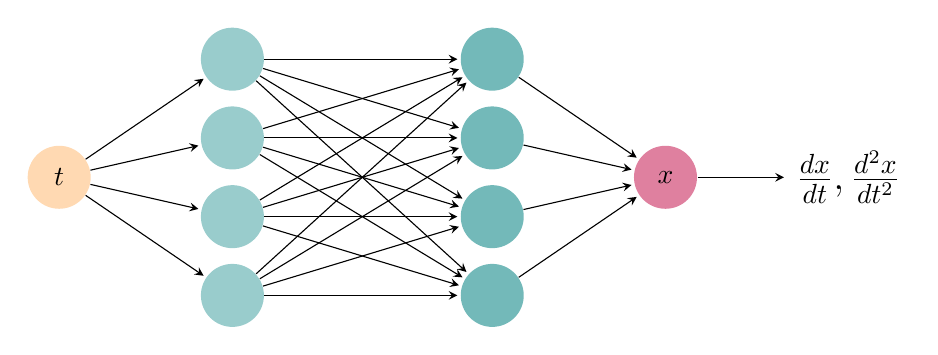
\begin{tikzpicture}[>=stealth, x=2.2cm, y=1cm]
\centering
% Parameters
\def\inputnum{1}
\def\hiddennum{4}
\def\outputnum{1}

% === Input Layer ===
\foreach \i in {1,...,\inputnum}{
  \node[circle, minimum size=8mm, fill=orange!30] 
    (Input-\i) at (0,-\i-1) {$t$};
}

% === Hidden Layer 1 ===
\foreach \i in {1,...,\hiddennum}{
  \node[circle, minimum size=8mm, fill=teal!40] 
    (HiddenA-\i) at (1,-\i + 0.5) {};
}

% === Hidden Layer 2 ===
\foreach \i in {1,...,\hiddennum}{
  \node[circle, minimum size=8mm, fill=teal!55] 
    (HiddenB-\i) at (2.5,-\i + 0.5) {};
}



% === Output Layer ===
\foreach \i in {1,...,\outputnum}{
  \node[circle, minimum size=8mm, fill=purple!50]
    (Output-\i) at (3.5,-\i-1) {$x$};
}

% === Connections ===
% Input → Hidden 1
\foreach \i in {1,...,\inputnum}{
  \foreach \j in {1,...,\hiddennum}{
    \draw[->, shorten >=1pt] (Input-\i) -- (HiddenA-\j);
  }
}

% Hidden 1 → Hidden 2
\foreach \i in {1,...,\hiddennum}{
  \foreach \j in {1,...,\hiddennum}{
    \draw[->, shorten >=1pt] (HiddenA-\i) -- (HiddenB-\j);
  }
}



% Hidden 3 → Output
\foreach \i in {1,...,\hiddennum}{
  \foreach \j in {1,...,\outputnum}{
    \draw[->, shorten >=1pt] (HiddenB-\i) -- (Output-\j);
  }
}
% Outputs
 \foreach \i in {1,...,\outputnum} { \draw[->, shorten >=1pt] 

 (Output-\i) -- ++(0.7,0) node[right]{\Large$\frac{dx}{dt} , \frac{d^2 x}{dt^2}$}; }

\end{tikzpicture}
\pause
$$ \text{Loss} = \frac{1}{N}\sum_{i}^{N}\left(x_{\text{nn}}(t_i)- x_{\text{true}}(t_i)\right)^2 + \frac{1}{M}\sum_{j}^{M}\left(\left[m\frac{d^2}{dt^2}+\mu\frac{d}{dt}+k\right]x_{\text{nn}}(t_j)\right)^2$$
\pause
  \begin{figure}
    \includegraphics[width=0.7\linewidth]{images/pinn/pinn-0.jpg}
\end{figure}
  \end{center}
\end{frame}

% \begin{frame}{PINN}
%   \begin{center}
%       \begin{tikzpicture}[>=stealth, x=2.2cm, y=1cm]
% \centering
% % Parameters
% \def\inputnum{1}
% \def\hiddennum{4}
% \def\outputnum{1}

% % === Input Layer ===
% \foreach \i in {1,...,\inputnum}{
%   \node[circle, minimum size=8mm, fill=orange!30] 
%     (Input-\i) at (0,-\i-1) {$t$};
% }

% % === Hidden Layer 1 ===
% \foreach \i in {1,...,\hiddennum}{
%   \node[circle, minimum size=8mm, fill=teal!40] 
%     (HiddenA-\i) at (1,-\i + 0.5) {};
% }

% % === Hidden Layer 2 ===
% \foreach \i in {1,...,\hiddennum}{
%   \node[circle, minimum size=8mm, fill=teal!55] 
%     (HiddenB-\i) at (2.5,-\i + 0.5) {};
% }



% % === Output Layer ===
% \foreach \i in {1,...,\outputnum}{
%   \node[circle, minimum size=8mm, fill=purple!50]
%     (Output-\i) at (3.5,-\i-1) {$x$};
% }

% % === Connections ===
% % Input → Hidden 1
% \foreach \i in {1,...,\inputnum}{
%   \foreach \j in {1,...,\hiddennum}{
%     \draw[->, shorten >=1pt] (Input-\i) -- (HiddenA-\j);
%   }
% }

% % Hidden 1 → Hidden 2
% \foreach \i in {1,...,\hiddennum}{
%   \foreach \j in {1,...,\hiddennum}{
%     \draw[->, shorten >=1pt] (HiddenA-\i) -- (HiddenB-\j);
%   }
% }



% % Hidden 3 → Output
% \foreach \i in {1,...,\hiddennum}{
%   \foreach \j in {1,...,\outputnum}{
%     \draw[->, shorten >=1pt] (HiddenB-\i) -- (Output-\j);
%   }
% }
% % Outputs
%  \foreach \i in {1,...,\outputnum} { \draw[->, shorten >=1pt] (Output-\i) -- ++(0.7,0) node[right]{\Large$\frac{dx}{dt} , \frac{d^2 x}{dt^2}$}; }

% \end{tikzpicture}
% $$ \text{Loss} = \frac{1}{N}\sum_{i}^{N}\left(x_{\text{nn}}(t_i)- x_{\text{true}}(t_i)\right)^2 + \frac{1}{M}\sum_{j}^{M}\left(\left[m\frac{d^2}{dt^2}+\mu\frac{d}{dt}+k\right]x_{\text{nn}}(t_j)\right)^2$$

%   \begin{figure}
% \animategraphics[loop, autoplay, width=0.7\linewidth]{18}{images/pinn/pinn-}{0}{132}
% \end{figure}
%   \end{center}
% \end{frame}

\begin{frame}{Forward problem}
  Solving a differential equation by knowing only the initial and or boundary conditions and the goal is to infer them from partial or indirect data.
  \pause
  \begin{center}
    $$ \text{Loss} = \left(x_{\text{nn}}(t=0)-1\right)^2 +\lambda_1\left(\frac{dx_{\text{nn}}}{dt}(t=0)\right)^2 +\frac{\lambda_2}{N}\sum_{j}^{N}\left(\left[m\frac{d^2}{dt^2}+\mu\frac{d}{dt}+k\right]x_{\text{nn}}(t_j)\right)^2$$
  \end{center}
  \pause
    \begin{figure}
      \includegraphics[width=0.7\linewidth]{images/forward/step_0.png}
\end{figure}
\end{frame}

% \begin{frame}{Forward problem}
%   Solving a differential equation by knowing only the initial and or boundary conditions and the goal is to infer them from partial or indirect data.
%   \begin{center}
%     $$ \text{Loss} = \left(x_{\text{nn}}(t=0)-1\right)^2 +\lambda_1\left(\frac{dx_{\text{nn}}}{dt}(t=0)\right)^2 +\frac{\lambda_2}{N}\sum_{j}^{N}\left(\left[m\frac{d^2}{dt^2}+\mu\frac{d}{dt}+k\right]x_{\text{nn}}(t_j)\right)^2$$
%   \end{center}
%     \begin{figure}
% \animategraphics[loop, autoplay, width=0.7\linewidth]{15}{images/forward/step_}{0}{100}
% \end{figure}
% \end{frame}

\begin{frame}{Inverse problem}
  In an inverse problem, the equation form is known, but some parts of it are unknown and the goal is to infer them from partial or indirect data.
  \pause
  \begin{center}
      $$ \text{Loss} = \frac{\lambda}{N}\sum_{i}^{N}\left(x_{\text{nn}}(t_i)- x_{\text{true}}(t_i)\right)^2 + \frac{1}{M}\sum_{j}^{M}\left(\left[m\frac{d^2}{dt^2}+\mu\frac{d}{dt}+k\right]x_{\text{nn}}(t_j)\right)^2$$

  \end{center}
  \pause
\begin{figure}[htbp]
  \centering
  % --- انیمیشن در سمت چپ ---
  \begin{minipage}[b]{0.66\textwidth}
    \centering
    \includegraphics[width=\linewidth]{images/inverse/frame_0.png}
  \end{minipage}
  \hfill
  % --- تصویر در سمت راست ---
  \begin{minipage}[b]{0.32\textwidth}
    \centering
    % \includegraphics[width=\linewidth]{images/Screenshot 2025-11-03 164745.png}
  \end{minipage}

\end{figure}

\end{frame}

% \begin{frame}{Inverse problem}
%   In an inverse problem, the equation form is known, but some parts of it are unknown and the goal is to infer them from partial or indirect data.
%   \begin{center}
%       $$ \text{Loss} = \frac{\lambda}{N}\sum_{i}^{N}\left(x_{\text{nn}}(t_i)- x_{\text{true}}(t_i)\right)^2 + \frac{1}{M}\sum_{j}^{M}\left(\left[m\frac{d^2}{dt^2}+\mu\frac{d}{dt}+k\right]x_{\text{nn}}(t_j)\right)^2$$

%   \end{center}

%   \begin{figure}[htbp]
%   \centering
%   % --- انیمیشن در سمت چپ ---
%   \begin{minipage}[b]{0.66\textwidth}
%     \centering
%     \animategraphics[loop,autoplay,width=\linewidth]{15}{images/inverse/frame_}{0}{100}
%   \end{minipage}
%   \hfill
%   % --- تصویر در سمت راست ---
%   \pause
%   \begin{minipage}[b]{0.32\textwidth}
%     \centering

%     \includegraphics[width=\linewidth]{images/Screenshot 2025-11-03 164745.png}
%   \end{minipage}

%   \end{figure}
% \end{frame}

\begin{frame}{PINN for solving Vlasov-Poisson equation}
        \begin{center}
        \begin{figure}
            \includegraphics[width=0.9\textwidth]{images/Screenshot 2025-11-06 200539.png}
        \end{figure}
    \end{center}
\end{frame}